\documentclass[a4paper, 12pt]{article}
% \newenvironment{inblk}{\begin{list}{}{\vspace*{-2mm}\setlength{\leftmargin}{10mm
% }}\item }{\vspace*{-2mm}\end{list}}
% \setlength{\parindent}{0pt}
% \setlength{\parskip}{2mm}
\usepackage{tabularx}
\usepackage[document]{ragged2e}
\usepackage{multirow}
\usepackage{changepage}
\usepackage{hyperref}
\usepackage{setspace}
\renewcommand{\baselinestretch}{1}
\usepackage{changepage}
\usepackage[usenames,dvipsnames,svgnames,table]{xcolor}
\usepackage{graphicx}
\usepackage[ampersand]{easylist}
\graphicspath{ {img/} }
%\textwidth=12.5cm
%\usepackage[document]{ragged2e}

\begin{document}

\begin{center}
\bfseries{ {\Large {CSSE1001}}\\
Semester 1, 2015\\
Assignment 3 - Instant Messenger Topic Suggestion\\}
\end{center}

\section{Introduction}
An instant messenger (commonly referred to as an `IM') is
a program that facilitates synchronous communication between two or more
clients over a network.\\[0.5\baselineskip]
There are many well-known implementations of IM systems that you may already be
familiar with, for example:
{\center
\begin{tabular}{p{0.2\linewidth} p{0.7\linewidth}}
\texttt{Facebook IM} & An IM system integrated into the facebook site.
\\[0.5\baselineskip]
\texttt{irssi} & A terminal-based IM for UNIX systems that uses the IRC
communication protocol.\\
[0.5\baselineskip]
\texttt{Skype IM Service} & A stand-alone IM application using a propietary, 
closed source network infrastructure.\\
[0.5\baselineskip]
\end{tabular}}
\\[\baselineskip]

You may choose to take inspiration from some of the elements of these
applications in your own assignments.\\[0.5\baselineskip]


\section{System Topology}
One of the largest design decisions you are likely to face when constructing an
instant messenger is how to structure communication between clients.\\
There are many possible ways to structure an instant messaging service. Whilst
there is no single `correct' way to do this, some methods are more ideal than
others. A few simplistic system topologies have been briefly outlined for you.
Please note that this list is by no means exhaustive. You should not feel
restricted by these suggestions.

\subsection{Peer-To-Peer Using a Name Server}
A \emph{Name Server} is a program with an IP address and port number known
by each messenger client. When one client wishes to begin a communication it
requests the IP address and port number of the other client process from the
Name Server, allowing a peer-to-peer connection to begin (see Figure 1).\\
\begin{center}
\begin{figure}[ht]
\centering
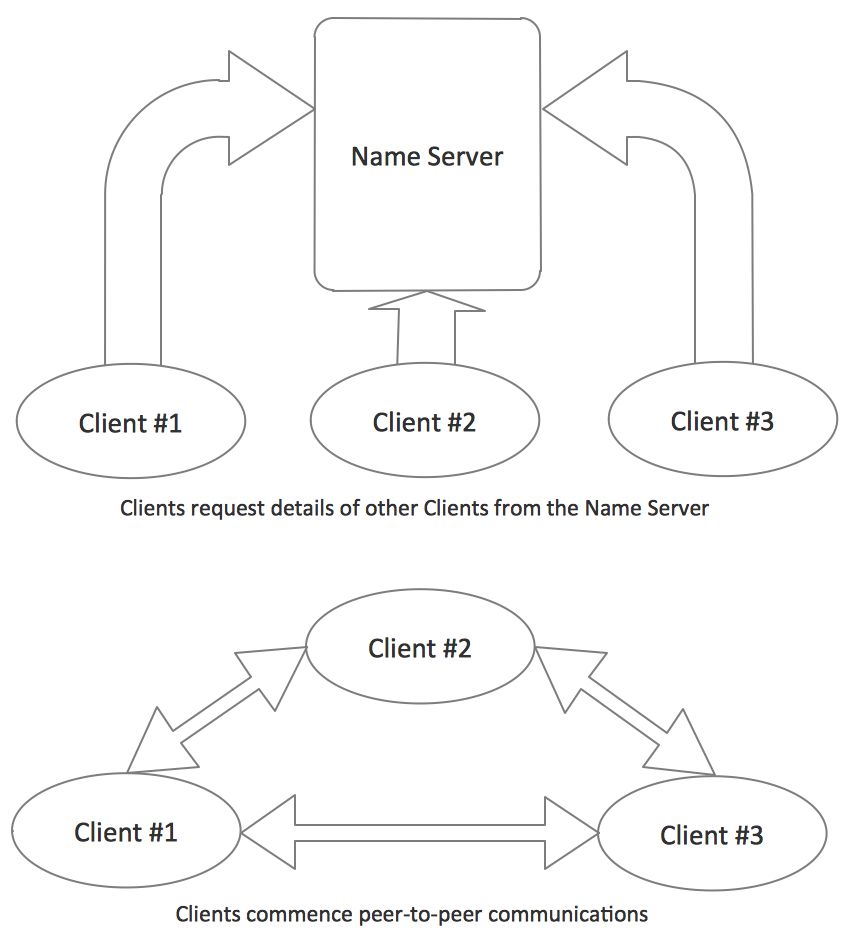
\includegraphics[scale=0.75]{p2p_topology}
\caption{Simplified Peer-to-Peer network topology}
\end{figure}
\end{center}


\subsection{Central Server Topology}
A program that contains address information for all active clients acts as a
`postal service' for messages between clients. That is, if client A is
communicating with client B, client A would send a message to the IM server
and the IM server would consequently send the message to client B (see Figure
2). This configuration requires the client processes to register themselves
with the IM server prior to commencing any other communications.
\begin{figure}
\centering
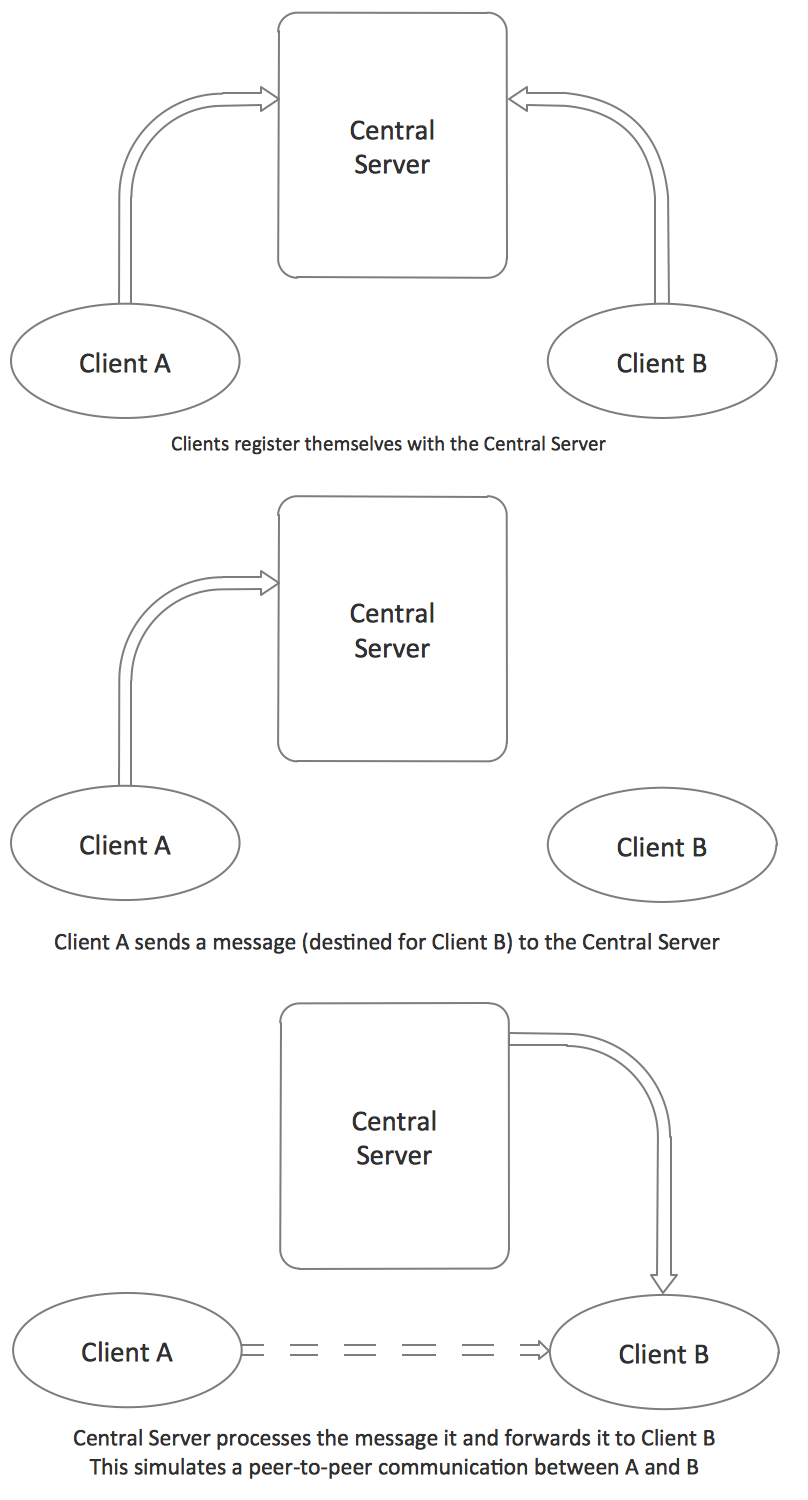
\includegraphics[scale=0.75]{central_server_topology}
\caption{Simplified central server network topology}
\end{figure}


\subsection{Publish/Subscribe Message Transport Topologies}
Messages can be broadcast to a number of client processes simultaneously
by using a publish/subscribe transport system such as MQTT (see 
\href{http://mqtt.org/}{\texttt{mqtt.org/}} for protocol documentation).\\
This configuration involves a number of clients \emph{subscribing} to a process
and receiving all messages \emph{published} to that same location by other
clients (see Figure 3).
\begin{figure}[h]
\centering
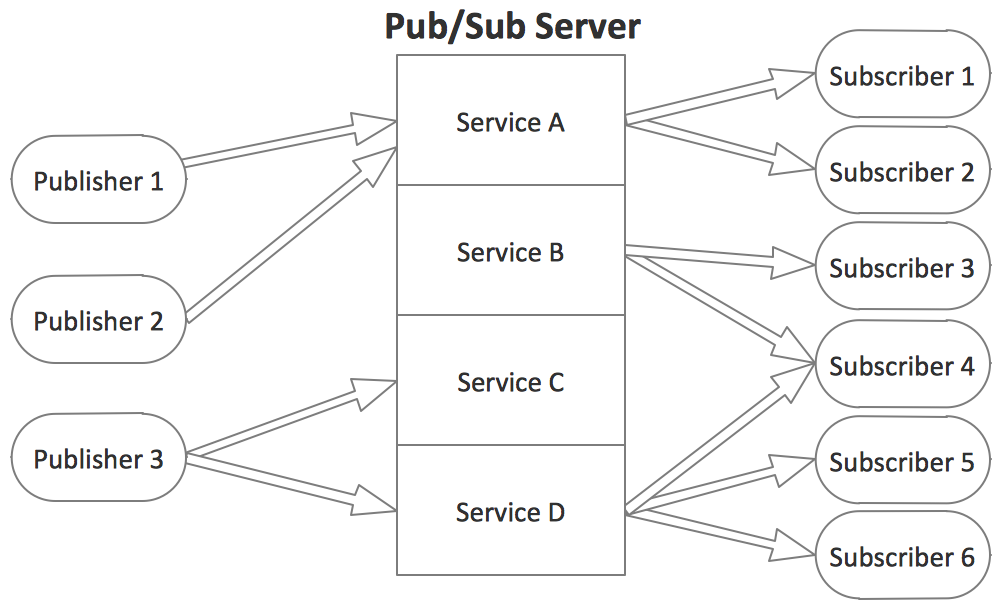
\includegraphics[scale=0.75]{ps_topology}
\caption{Simplified publish/subscribe system topology}
\end{figure}

\pagebreak


\section{Expecations}
As is eluded to in the Assignment 3 task sheet, the more complexity you\\
add to your assignment the higher your assignment's rank. Since the\\design
decisions involved in this assignment are to be yours, a number of\\possible 
features for inclusion in your assignment have been included. 
\\[0.5\baselineskip]
It should be noted that this list is neither exhaustive nor compulsory.
You may choose to implement any number of these features as well as ones not 
included here.

\subsection{Basic Features}
\begin{itemize}
\item Some form of User Interface
    \begin{itemize}
    \item Text interface (similar to the IRSSI client)
    \item Graphical user interface (similar to the \emph{Skype} interface)
    \end{itemize}
\item Capactiy to hold concurrent conversations
    \begin{itemize}
    \item This may require knowledge of some concurrency programming
    techniques (see section 4.3)
    \end{itemize}
\item Client addressing system (i.e. some form of an address book)
\end{itemize}

\subsection{Advanced Features}
\begin{itemize}
\item Asynchronous communication between hosts
    \begin{itemize}
    \item Messages sent to an unavailable host will be delivered once the host
    is next visible
    \end{itemize}
\item Multi-host conversations
    \begin{itemize}
    \item Allow conversations between three or more different clients
    \end{itemize}
\item Persistent conversations between login sessions
    \begin{itemize}
    \item Maintain a history of conversations so that a conversation is not
    lost once a conversation session is terminated
    \end{itemize}
\item Image and file transfer
    \begin{itemize}
    \item This may require research of file transfer protocols such as \emph{ftp} and
    \emph{http}
    \end{itemize}
\end{itemize}

\pagebreak
\section{Resources}
You will need to use a number of resources in order to implement this
assignment. Some possibly useful libraries include: 

\subsection{Networking Resources}
\subsubsection*{socket.socket}
Comes packaged as a part of the standard Python 3 distribution. There is
extensive documentation and examples on how to use Python sockets online. One
such resource can be seen at \href{https://docs.python.org/3/library/socket.html}{https://docs.python.org/3/library/socket.html}.

\subsubsection*{paho-mqtt}
\texttt{paho-mqtt} is an implementation of the MQTT protocol for Python.
Installation guidlines can be found at
\href{https://pypi.python.org/pypi/paho-mqtt}
{https://pypi.python.org/pypi/paho-mqtt}. Basic usage instructions can also be
found here.

\subsection{User Interface Resources}
\subsubsection*{TkInter}
\texttt{TkInter} will come installed as a part of the standard Python 3
distribution. This is the library used in CSSE1001 to teach Graphical User
Interfaces. Guidance on using this resource can be found in the course notes as
well as online.

\subsubsection*{PyQt4}
PyQt4 is a popular GUI library written by Riverbank Computing Limited. It has a
large community following and can be installed for Windows from the Riverbank
website (\href{http://www.riverbankcomputing.com/software/pyqt/download}
{www.riverbankcomputing.com/software/pyqt/download}). OS X systems can install
PyQt4 by installing homebrew (\href{http://brew.sh}{brew.sh}) and running the following commands in a terminal window:\\[0.5\baselineskip]
\begin{adjustwidth}{50pt}{}
\texttt{brew install sip --with-python3}\\
\texttt{brew install pyqt --with-python3}\\[0.5\baselineskip]
\end{adjustwidth}

\pagebreak

\subsection{Concurrency Resources}
One of the simplest methods of achieving concurrency is through the use of 
\emph{multi-threading}.\\
Threads are a service provided by some operating systems to user\\ applications
that allow elements of a program to be run concurrently. Some\\ implementations
of instant messengers may require such services.\\[0.5\baselineskip]
Thankfully, a threading library is included in the standard Python 3.4\\
distribution. This library, named \texttt{threading}, is well documented at 
locations such as the Python website: 
(\href{https://docs.python.org/3/library/threading.html}
{https://docs.python.org/3/library/threading.html}). Example implementations of
multithreaded applications (such as the examples found at 
\href{http://pymotw.com/2/threading}{http://pymotw.com/2/threading/}) are also 
easily accessible.


\end{document}
